\documentclass[11pt,a4paper]{article}

\usepackage[utf8]{inputenc}
\usepackage[ngerman]{babel}
\usepackage{amsmath}
\usepackage{amsthm}
\usepackage{graphicx}
\graphicspath{ {./images/} }

\title{ARJA: Automated Repair of Java Programs via
Multi-Objective Genetic Programming \\[0.5em] \large{Seminar zu ``Machine Learning in Software Eningeering'' \\[0.5em]} }

\author{Paul Groß, David Riemer, Felix Groß}

\date{Sommersemester 2023}

\begin{document}
\maketitle

\section{Einführung in die Funktionsweise von ARJA}
\section{Nutzung des Softwaresystems}
Dieser Abschnitt befasst sich mit dem Einsatz von ARJA in SoftwareEntwicklungsprojekten. Es soll gezeigt werden, unter welchen Umst¨anden
es sich lohnt auf automatische Programmreparatur zuruckzugreifen und wie ¨
der Workflow fur die Entwicklenden Personen des Projekts aussieht.
\subsection{Einsatzfälle von ARJA in Entwicklungsprojekten Korrektur}
Als Entwickler eines Softwareprojekts ist es in allen Phasen des Softwareentwicklungsprozesses wichtig, eine funktionsfähige Software zu entwickeln/warten.

Test-getriebene Entwicklung ist ein agiler Softwareentwicklungsansatz, bei dem Tests vor der eigentlichen Implementierung des Codes geschrieben werden. Der Ansatz besteht aus einem iterativen und inkrementellen Entwicklungszyklus, der aus den folgenden Schritten besteht:

Zuerst werden die Testfälle anhand der Anforderungen des Programms beschrieben und anschließend programmiert; anschließend wird der Code des zu schreibenden Programms so lange geändert, bis das Programm alle gegebenen Tests besteht.

Bei der Entwicklung eines komplexen Programms kann es jedoch vorkommen, dass Tests, welche bei Erstentwicklung noch fehlerfrei abliefen nun Fehler verursachen. Natürlich kann dies auch der Fall sein, wenn der Entwickler oder das Entwicklerteam sich dazu entscheidet Test erst nach dem Ausbau der Software zu verfassen. Nun ist es sinnvoll zu überlegen in welchen Anwendungsfällen der Einsatz für eines automatischen repair-Programms zweckmäßig ist und wann man lieber darauf verzichten sollte.

\subsubsection{Entscheidung anhand äußerlicher Sachverhalte}

Einer der wichtigsten Aspekte in der Softwareentwicklung ist die Zeit. Werden bestimmte Deadlines für Bugfixes, Features, etc. nicht eingehalten kann dies meist verheerende Folgen im Prozess der Softwareentwicklung haben. Wenn man als Entwickler also unter Zeitdruck steht, kann die Verwendung automatischer Reparaturwerkzeuge(besonders von ARJA)den Zeitaufwand für das manuelle Beheben von Bugs reduzieren. Dadurch hat der Entwickler mehr Zeit, sich wichtigeren Aufgaben zu widmen.

Ein weiterer Fall für den Einsatz von ARP ist der Fall der Ressourcenbeschränkungen: Wenn dem Entwickler das erforderliche Fachwissen oder die Ressourcen fehlen, um bestimmte Fehler manuell zu beheben, können automatische Reparaturwerkzeuge eine nützliche Alternative sein. Sie können ihm unter anderem dabei helfen, Fehler zu korrigieren, für die er möglicherweise nicht über das erforderliche Wissen oder die erforderliche Erfahrung verfügt. Hier sollte man jedoch Vorsicht wallten lassen. Wie man in den kommenden Abschnitten sieht, sind ARPs, inklusive ARJA doch fehleranfällig. Der Entwickler sollte sicher gehen, dass der durch das Programm erstellte Patch auch wirklich den Bug im System gefixed hat und kein Fehler, z. B. in Form von overfitting zu Stande gekommen ist.

\subsubsection{Entscheidung anhand des Codes}

Abgesehen von Kriterien der äußerlichen Natur ist es natürlich umso wichtiger Code spezifische Sachverhalte zu nennen:

Wenn zum Beispiel ein Test gehäuft fehlschlägt, ist es gut möglich, dass ein ARP besser in der Lage ist das Fehlermuster zu erkennen und zu korrigieren. Dies liegt in der Natur des Machine Learnings.

Außerdem sollte man bei großen Codebasen abwägen, ob die manuelle Fehlersuche optimaler ist als die Verwendung von ARPs und anschließende Analyse des entstandenen Patches. Fehlende Code-Kommentare, redundanter code, Nichteinhalten von den ISO-Normen und viele weitere Faktoren können Gründe dafür sein, wieso das Programm für einen Entwickler nur schwierig lesbar ist. Da ARJA das Programm aber nicht wie ein Mensch übergeht sonders als einen „abstract syntax tree“ repräsentiert, kann es hier durchaus effizienter sein ein ARP anzuwenden, gerade bei immer komplexer werdenden Softwaresystemen. Daran anschließen kann man die Legacy-Code-Wartung:

Bei der Wartung von Legacy Code, der oft wenig oder keine Dokumentation aufweist, können automatische Reparaturwerkzeuge helfen, Fehler zu finden und zu beheben. Sie können aber auch bei der Verbesserung der Codequalität und -strukturierung älterer Codebasen unterstützen.

Letzten Endes liegt es in der Hand des Entwicklers oder des Entwicklerteams zu entscheiden, ob ein ARP eingesetzt werden sollte oder nicht. Das auf den ersten Blick durchaus effizientere Bugfixing sollte unter keinen Umständen unkontrolliert bleiben und kann unter Umständen mehr Arbeit nach sich ziehen, als ein manuelles Fixen des Codes.
\subsection{Bedienung des Systems als Entwickler}
Figur x beschreibt ein typisches Ablaufszenario für den Einsatz von ARJA als Entwickler.


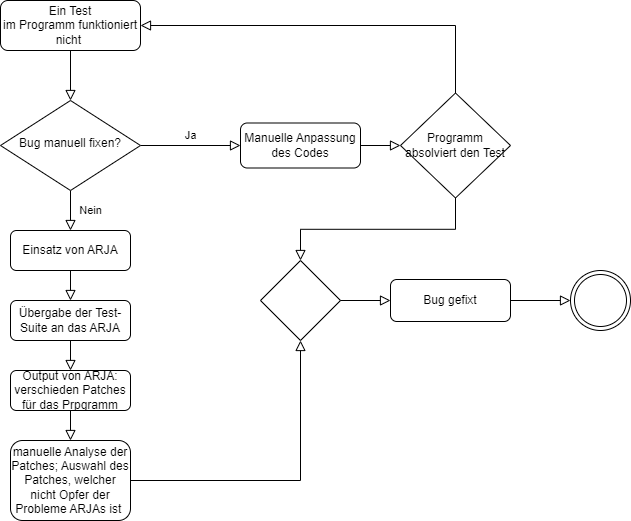
\includegraphics[width=50mm,scale=0.5]{ablauf.png}

Es fällt auf, dass der Einsatz eines automatisierten Programms für die Fehlerbehebung auf den ersten Blick zwar als die deutlich sparsamere Variante, aber in manchen Einzelfällen einige Schritte mit sich bringt, welche eventuell komplexer und aufwändiger sind als die manuelle Behebung des Problems.






\bibliographystyle{abbrv}
\bibliography{seminar}

\end{document}
